\documentclass[11pt]{article}
\usepackage{minted, tikz, blindtext}
\usepackage{amsfonts, amssymb, amsmath, float}
\usepackage{enumerate, esint, nicefrac, algorithm2e}
\parindent 0px
\date{September 28, 2023}
\title{CS301 :: Midterm 1}
\author{Ryan Magdaleno\\71/80 Score}

% Helpful ::
% \line(1,0){358px}
\begin{document}
\maketitle

%%%%%%%%%%%%%%%%%%%%%%%%%%%%%%%%%%%%%%%%%%%%%%%%%%%%%%%%%%%%%%%%%%%%%%%%%%%%%%%%%%%%%%%%%

\textbf{Problem 1: Multiple Choice}

\vspace{5px}\textbf{Solution ::} 
\begin{enumerate}[a)]
\item Which of the following constraints exists for the transition function in an NFA
5-tuple. \\
$\delta : Q\times (\Sigma\cup\epsilon)\longrightarrow P(Q)$.
\item Given that $A$ and $B$ are regular languages, which of the following are
not regular. \\ $A^nB^n$.
\item Which of the following languages is finite? \\
$L_b = \{w\in\{0,1\}^* : |w|\le 20\}$.
\item From the pumping lemma, any string $s$ with more than $p$ characters can
be partitioned into $xyz$. Identify the property of $x,y,z$ below which is true. \\
$z$ must be a suffix of $s$.
\item For a given DFA $M$, which of the following can be infinite? \\
The language it decides.
\item All finite languages are regular. \\ True.
\item Which of the following is a base case for the recursive structure of regular
expressions? \\ $\emptyset$ : The empty set.
\item Which of the following languages are not regular? \\
$L_a = \{w\in\{0,1\}^* : w\text{ has at least three zeros for every one}\}$.
\end{enumerate}
\pagebreak

%%%%%%%%%%%%%%%%%%%%%%%%%%%%%%%%%%%%%%%%%%%%%%%%%%%%%%%%%%%%%%%%%%%%%%%%%%%%%%%%%%%%%%%%%

\textbf{Problem 2: Short Answer}
\begin{enumerate}[a)]
\item
Give an example of an infinitely large binary language. \\
\vspace{5px}\textbf{Solution ::}
$$L=(01)^*$$

\line(1,0){343px}

\item
Given an NFAs $M_A, M_B$ which decide $L_A, L_B$ respectively, describe how
to generate an NFA which decides their concatenation, $L_AL_B$. \\
\vspace{5px}\textbf{Solution ::} \\
Given $M_A$ and $M_B$ we can make the concatenation $L_AL_B$ by adding
epsilons from the final states of NFA $M_A$ to the start state of NFA $M_B$.
We must then make the start state of $M_B$. We must then make the start state
of $M_B$ become a normal state, the final states of $M_A$ normal.
\begin{align*}
    L(L_A)\circ L(L_B) &= \{xy \,|\, x\in L(L_A) \cap y\in L(L_B)\} \\
    Q &= \{Q_A\cup Q_B\} \\
    \Sigma &= \Sigma_A = \Sigma_B \\
    q_0 &= q_{0_A} \\
    F &= \{F_B\} \\
    \delta &= \delta_A\cup\delta_B\cup(F_A,\epsilon\longrightarrow q_{0_B})
\end{align*}
\line(1,0){343px}

\item
Give the 5-tuple for a DFA which accepts the empty language. \\
Let $\Sigma = \{0, 1\}$ \\
\vspace{5px}\textbf{Solution ::}
\begin{align*}
    Q &= \{q_0\} \\
    \Sigma &= \{0, 1\} \\
    q_0 &= q_0 \\
    F &= \emptyset \\
    \delta &= \{(q_0, 0)\longrightarrow q_0 \,|\, (q_0, 1)\longrightarrow q_0\}
\end{align*}
\end{enumerate}
\pagebreak

%%%%%%%%%%%%%%%%%%%%%%%%%%%%%%%%%%%%%%%%%%%%%%%%%%%%%%%%%%%%%%%%%%%%%%%%%%%%%%%%%%%%%%%%%

\textbf{Problem 3: NFA to DFA} \\
Consider the following NFA $M$: 
\begin{center}
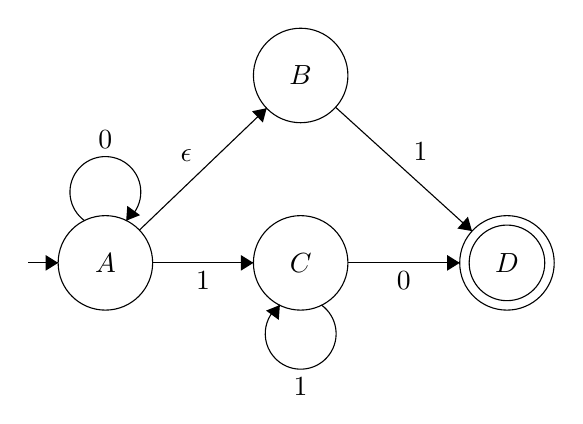
\begin{tikzpicture}[scale=0.2]
\tikzstyle{every node}+=[inner sep=0pt]
\draw [black] (19.2,-27.5) circle (3);
\draw (19.2,-27.5) node {$A$};
\draw [black] (31.6,-15.6) circle (3);
\draw (31.6,-15.6) node {$B$};
\draw [black] (31.6,-27.5) circle (3);
\draw (31.6,-27.5) node {$C$};
\draw [black] (44.7,-27.5) circle (3);
\draw (44.7,-27.5) node {$D$};
\draw [black] (44.7,-27.5) circle (2.4);
\draw [black] (14.3,-27.5) -- (16.2,-27.5);
\fill [black] (16.2,-27.5) -- (15.4,-27) -- (15.4,-28);
\draw [black] (17.877,-24.82) arc (234:-54:2.25);
\draw (19.2,-20.25) node [above] {$0$};
\fill [black] (20.52,-24.82) -- (21.4,-24.47) -- (20.59,-23.88);
\draw [black] (21.36,-25.42) -- (29.44,-17.68);
\fill [black] (29.44,-17.68) -- (28.51,-17.87) -- (29.2,-18.59);
\draw (24.33,-21.07) node [above] {$\epsilon$};
\draw [black] (33.82,-17.62) -- (42.48,-25.48);
\fill [black] (42.48,-25.48) -- (42.22,-24.57) -- (41.55,-25.32);
\draw (39.21,-21.06) node [above] {$1$};
\draw [black] (34.6,-27.5) -- (41.7,-27.5);
\fill [black] (41.7,-27.5) -- (40.9,-27) -- (40.9,-28);
\draw (38.15,-28) node [below] {$0$};
\draw [black] (22.2,-27.5) -- (28.6,-27.5);
\fill [black] (28.6,-27.5) -- (27.8,-27) -- (27.8,-28);
\draw (25.4,-28) node [below] {$1$};
\draw [black] (32.923,-30.18) arc (54:-234:2.25);
\draw (31.6,-34.75) node [below] {$1$};
\fill [black] (30.28,-30.18) -- (29.4,-30.53) -- (30.21,-31.12);
\end{tikzpicture}
\end{center}

Give the state diagram for a DFA that is equivalent to $M$. \\
\vspace{5px}\textbf{Solution ::}
\begin{center}
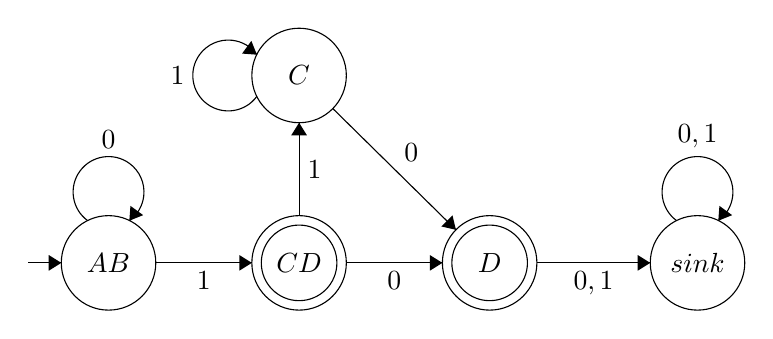
\begin{tikzpicture}[scale=0.2]
\tikzstyle{every node}+=[inner sep=0pt]
\draw [black] (16.1,-30.1) circle (3);
\draw (16.1,-30.1) node {$AB$};
\draw [black] (28.2,-30.1) circle (3);
\draw (28.2,-30.1) node {$CD$};
\draw [black] (28.2,-30.1) circle (2.4);
\draw [black] (28.2,-18.2) circle (3);
\draw (28.2,-18.2) node {$C$};
\draw [black] (40.3,-30.1) circle (3);
\draw (40.3,-30.1) node {$D$};
\draw [black] (40.3,-30.1) circle (2.4);
\draw [black] (53.5,-30.1) circle (3);
\draw (53.5,-30.1) node {$sink$};
\draw [black] (14.777,-27.42) arc (234:-54:2.25);
\draw (16.1,-22.85) node [above] {$0$};
\fill [black] (17.42,-27.42) -- (18.3,-27.07) -- (17.49,-26.48);
\draw [black] (11,-30.1) -- (13.1,-30.1);
\fill [black] (13.1,-30.1) -- (12.3,-29.6) -- (12.3,-30.6);
\draw [black] (19.1,-30.1) -- (25.2,-30.1);
\fill [black] (25.2,-30.1) -- (24.4,-29.6) -- (24.4,-30.6);
\draw (22.15,-30.6) node [below] {$1$};
\draw [black] (28.2,-27.1) -- (28.2,-21.2);
\fill [black] (28.2,-21.2) -- (27.7,-22) -- (28.7,-22);
\draw (28.7,-24.15) node [right] {$1$};
\draw [black] (31.2,-30.1) -- (37.3,-30.1);
\fill [black] (37.3,-30.1) -- (36.5,-29.6) -- (36.5,-30.6);
\draw (34.25,-30.6) node [below] {$0$};
\draw [black] (30.34,-20.3) -- (38.16,-28);
\fill [black] (38.16,-28) -- (37.94,-27.08) -- (37.24,-27.79);
\draw (35.32,-23.67) node [above] {$0$};
\draw [black] (25.52,-19.523) arc (-36:-324:2.25);
\draw (20.95,-18.2) node [left] {$1$};
\fill [black] (25.52,-16.88) -- (25.17,-16) -- (24.58,-16.81);
\draw [black] (43.3,-30.1) -- (50.5,-30.1);
\fill [black] (50.5,-30.1) -- (49.7,-29.6) -- (49.7,-30.6);
\draw (46.9,-30.6) node [below] {$0,1$};
\draw [black] (52.177,-27.42) arc (234:-54:2.25);
\draw (53.5,-22.85) node [above] {$0,1$};
\fill [black] (54.82,-27.42) -- (55.7,-27.07) -- (54.89,-26.48);
\end{tikzpicture}
\end{center}
\pagebreak

%%%%%%%%%%%%%%%%%%%%%%%%%%%%%%%%%%%%%%%%%%%%%%%%%%%%%%%%%%%%%%%%%%%%%%%%%%%%%%%%%%%%%%%%%

\textbf{Problem 4: NFA to REGEX} \\
Consider the following GNFA $M$. Give an equivalent GNFA w/out state $C$.
\begin{center}
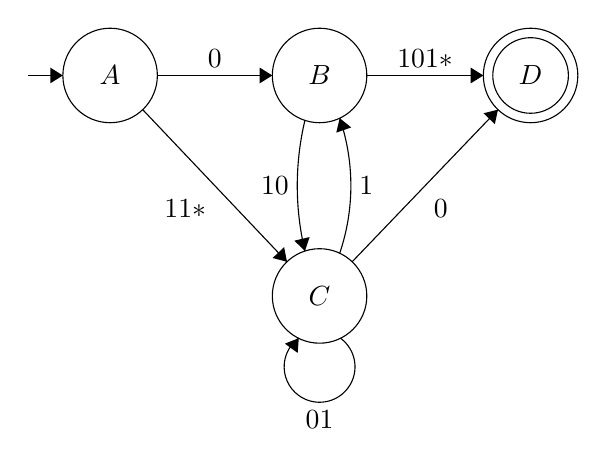
\begin{tikzpicture}[scale=0.2]
\tikzstyle{every node}+=[inner sep=0pt]
\draw [black] (20.3,-22.2) circle (3);
\draw (20.3,-22.2) node {$A$};
\draw [black] (33.6,-22.2) circle (3);
\draw (33.6,-22.2) node {$B$};
\draw [black] (33.6,-36.2) circle (3);
\draw (33.6,-36.2) node {$C$};
\draw [black] (47,-22.2) circle (3);
\draw (47,-22.2) node {$D$};
\draw [black] (47,-22.2) circle (2.4);
\draw [black] (23.3,-22.2) -- (30.6,-22.2);
\fill [black] (30.6,-22.2) -- (29.8,-21.7) -- (29.8,-22.7);
\draw (26.95,-21.7) node [above] {$0$};
\draw [black] (36.6,-22.2) -- (44,-22.2);
\fill [black] (44,-22.2) -- (43.2,-21.7) -- (43.2,-22.7);
\draw (40.3,-21.7) node [above] {$101*$};
\draw [black] (34.877,-24.908) arc (18.80126:-18.80126:13.319);
\fill [black] (34.88,-24.91) -- (34.66,-25.83) -- (35.61,-25.5);
\draw (36.09,-29.2) node [right] {$1$};
\draw [black] (32.669,-33.352) arc (-166.67036:-193.32964:18.008);
\fill [black] (32.67,-33.35) -- (32.97,-32.46) -- (32,-32.69);
\draw (31.68,-29.2) node [left] {$10$};
\draw [black] (35.67,-34.03) -- (44.93,-24.37);
\fill [black] (44.93,-24.37) -- (44.01,-24.6) -- (44.73,-25.29);
\draw (40.83,-30.67) node [right] {$0$};
\draw [black] (22.37,-24.37) -- (31.53,-34.03);
\fill [black] (31.53,-34.03) -- (31.35,-33.1) -- (30.62,-33.79);
\draw (26.42,-30.67) node [left] {$11*$};
\draw [black] (34.923,-38.88) arc (54:-234:2.25);
\draw (33.6,-43.45) node [below] {$01$};
\fill [black] (32.28,-38.88) -- (31.4,-39.23) -- (32.21,-39.82);
\draw [black] (15.1,-22.2) -- (17.3,-22.2);
\fill [black] (17.3,-22.2) -- (16.5,-21.7) -- (16.5,-22.7);
\end{tikzpicture}
\end{center}
\vspace{5px}\textbf{Solution ::}
\begin{center}
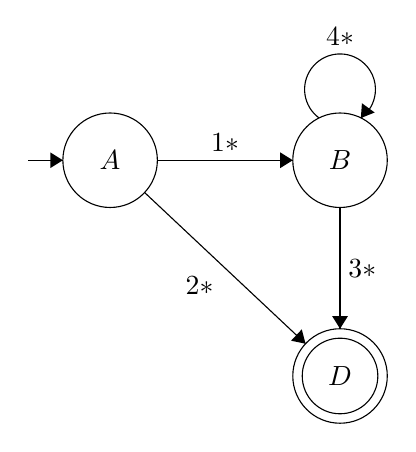
\begin{tikzpicture}[scale=0.2]
\tikzstyle{every node}+=[inner sep=0pt]
\draw [black] (20.4,-20.3) circle (3);
\draw (20.4,-20.3) node {$A$};
\draw [black] (35,-20.3) circle (3);
\draw (35,-20.3) node {$B$};
\draw [black] (35,-34) circle (3);
\draw (35,-34) node {$D$};
\draw [black] (35,-34) circle (2.4);
\draw [black] (23.4,-20.3) -- (32,-20.3);
\fill [black] (32,-20.3) -- (31.2,-19.8) -- (31.2,-20.8);
\draw (27.7,-19.8) node [above] {$1*$};
\draw [black] (22.59,-22.35) -- (32.81,-31.95);
\fill [black] (32.81,-31.95) -- (32.57,-31.04) -- (31.89,-31.76);
\draw (26.08,-27.63) node [below] {$2*$};
\draw [black] (35,-23.3) -- (35,-31);
\fill [black] (35,-31) -- (35.5,-30.2) -- (34.5,-30.2);
\draw (35.5,-27.15) node [right] {$3*$};
\draw [black] (33.677,-17.62) arc (234:-54:2.25);
\draw (35,-13.05) node [above] {$4*$};
\fill [black] (36.32,-17.62) -- (37.2,-17.27) -- (36.39,-16.68);
\draw [black] (15.2,-20.3) -- (17.4,-20.3);
\fill [black] (17.4,-20.3) -- (16.6,-19.8) -- (16.6,-20.8);
\end{tikzpicture}
\end{center}
\begin{align*}
    1* &= 0\cup11^*(01)^*1 \\
    2* &= 11^*(01)^*0 \\
    3* &= 10(01)^*0\cup 101^*\\
    4* &= 10(01)^*1
\end{align*}
\pagebreak

%%%%%%%%%%%%%%%%%%%%%%%%%%%%%%%%%%%%%%%%%%%%%%%%%%%%%%%%%%%%%%%%%%%%%%%%%%%%%%%%%%%%%%%%%

\textbf{Problem 5: Regex to NFA} \\
Give the state diagram for an NFA which decies the language $L$. \\
$\Sigma = \{0,1\}$
$$L = 10(11)^*(000\cup 1)^*$$
\vspace{5px}\textbf{Solution ::}
\begin{center}
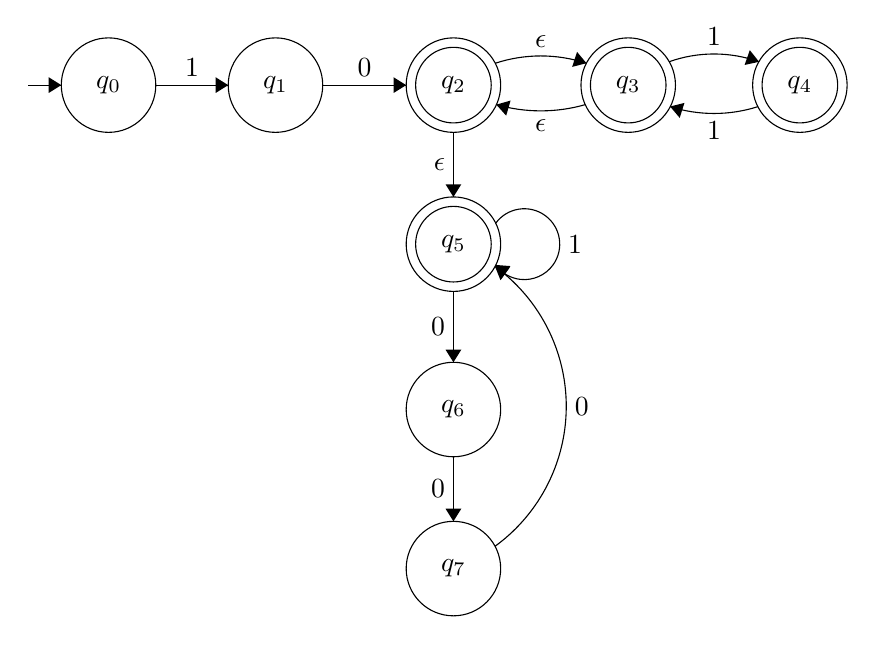
\begin{tikzpicture}[scale=0.2]
\tikzstyle{every node}+=[inner sep=0pt]
\draw [black] (18.2,-16.5) circle (3);
\draw (18.2,-16.5) node {$q_0$};
\draw [black] (28.8,-16.5) circle (3);
\draw (28.8,-16.5) node {$q_1$};
\draw [black] (40.1,-16.5) circle (3);
\draw (40.1,-16.5) node {$q_2$};
\draw [black] (40.1,-16.5) circle (2.4);
\draw [black] (51.2,-16.5) circle (3);
\draw (51.2,-16.5) node {$q_3$};
\draw [black] (51.2,-16.5) circle (2.4);
\draw [black] (62.1,-16.5) circle (3);
\draw (62.1,-16.5) node {$q_4$};
\draw [black] (62.1,-16.5) circle (2.4);
\draw [black] (40.1,-26.6) circle (3);
\draw (40.1,-26.6) node {$q_5$};
\draw [black] (40.1,-26.6) circle (2.4);
\draw [black] (40.1,-37.1) circle (3);
\draw (40.1,-37.1) node {$q_6$};
\draw [black] (40.1,-47.2) circle (3);
\draw (40.1,-47.2) node {$q_7$};
\draw [black] (13.1,-16.5) -- (15.2,-16.5);
\fill [black] (15.2,-16.5) -- (14.4,-16) -- (14.4,-17);
\draw [black] (21.2,-16.5) -- (25.8,-16.5);
\fill [black] (25.8,-16.5) -- (25,-16) -- (25,-17);
\draw (23.5,-16) node [above] {$1$};
\draw [black] (31.8,-16.5) -- (37.1,-16.5);
\fill [black] (37.1,-16.5) -- (36.3,-16) -- (36.3,-17);
\draw (34.45,-16) node [above] {$0$};
\draw [black] (42.746,-15.115) arc (108.32711:71.67289:9.235);
\fill [black] (48.55,-15.11) -- (47.95,-14.39) -- (47.64,-15.34);
\draw (45.65,-14.15) node [above] {$\epsilon$};
\draw [black] (48.479,-17.737) arc (-73.95736:-106.04264:10.235);
\fill [black] (42.82,-17.74) -- (43.45,-18.44) -- (43.73,-17.48);
\draw (45.65,-18.64) node [below] {$\epsilon$};
\draw [black] (53.79,-15.018) arc (109.66861:70.33139:8.497);
\fill [black] (59.51,-15.02) -- (58.92,-14.28) -- (58.59,-15.22);
\draw (56.65,-14.02) node [above] {$1$};
\draw [black] (59.443,-17.864) arc (-72.21685:-107.78315:9.146);
\fill [black] (53.86,-17.86) -- (54.47,-18.58) -- (54.77,-17.63);
\draw (56.65,-18.8) node [below] {$1$};
\draw [black] (40.1,-19.5) -- (40.1,-23.6);
\fill [black] (40.1,-23.6) -- (40.6,-22.8) -- (39.6,-22.8);
\draw (39.6,-21.55) node [left] {$\epsilon$};
\draw [black] (40.1,-29.6) -- (40.1,-34.1);
\fill [black] (40.1,-34.1) -- (40.6,-33.3) -- (39.6,-33.3);
\draw (39.6,-31.85) node [left] {$0$};
\draw [black] (40.1,-40.1) -- (40.1,-44.2);
\fill [black] (40.1,-44.2) -- (40.6,-43.4) -- (39.6,-43.4);
\draw (39.6,-42.15) node [left] {$0$};
\draw [black] (42.78,-25.277) arc (144:-144:2.25);
\draw (47.35,-26.6) node [right] {$1$};
\fill [black] (42.78,-27.92) -- (43.13,-28.8) -- (43.72,-27.99);
\draw [black] (42.736,-28.012) arc (54.00483:-54.00483:10.986);
\fill [black] (42.74,-28.01) -- (43.09,-28.89) -- (43.68,-28.08);
\draw (47.77,-36.9) node [right] {$0$};
\end{tikzpicture}
\end{center}
\pagebreak

%%%%%%%%%%%%%%%%%%%%%%%%%%%%%%%%%%%%%%%%%%%%%%%%%%%%%%%%%%%%%%%%%%%%%%%%%%%%%%%%%%%%%%%%%

\textbf{Problem 6: Non-Context-Free Proof} \\
Prove that the following language $L$ is irregular.
$$L = \{w\in\Sigma^* : w \text{ contains more 0's than 1's}\}$$
\vspace{5px}\textbf{Solution ::}

Let's assum $L$ is regular for the sake of contradiction. There must be some
DFA that decides $L$. Therefore there is a pumping length $p$.

Let $s = 1^p0^{p+1}$, $s$ can be partitioned into $xy^iz, i\ge 0$. \\
$x$ must be $1^\alpha$, $0\le\alpha\le p-\beta$. \\
$y$ must be $1^{i\beta}$, $1\le\beta < p - \alpha$. \\
$xy$ is within $p$. $\alpha + \beta\le p$.

If we pick $i=2$ we get the form $xyyz$ which is $\in L$. Therefore we get:
$$1^\alpha1^\beta1^{p-\beta-\alpha}0^{p+1} = 1^{p+\beta}0^{p+1}$$
However, we get the contradiction $p+\beta\ge p+1$. The original regular
language condition was that there were more 0s than 1s but because
$\beta$ must always be $\ge 1$ they will always be at least equal.

$\therefore L$ is not regular.
\end{document}